\documentclass[oneside]{book}

\usepackage{mathtools}
\usepackage{graphicx}
\usepackage[utf8]{inputenc}
\usepackage{float}
\usepackage{tabularx}
\usepackage[toc,page]{appendix}
\usepackage{gensymb}
\usepackage{subcaption}
\usepackage{tikz}
\usepackage{circuitikz}
\usepackage{array}
\usepackage{booktabs}
\usepackage{colortbl}
\usepackage{xcolor}
\usepackage{xfrac}
\usepackage{caption}

\usepackage[a4paper, inner=1.5cm, outer=3cm, top=3cm, 
bottom=3cm, bindingoffset=1cm]{geometry} 

\renewcommand{\thesubfigure}{\arabic{subfigure}}


\usepackage{fancyhdr}
\renewcommand{\chaptername}{Experiment}

\makeatletter
\def\pgf@circ@myvoltmeter@path#1{\pgf@circ@bipole@path{myvoltmeter}{#1}}
\tikzset{myvoltmeter/.style = {\circuitikzbasekey, /tikz/to
                               path=\pgf@circ@myvoltmeter@path}}
\pgfcircdeclarebipole{}{\ctikzvalof{bipoles/voltmeter/height}}{myvoltmeter}{\ctikzvalof{bipoles/voltmeter/height}}{\ctikzvalof{bipoles/voltmeter/width}}{
    \def\pgf@circ@temp{right}
    \ifx\tikz@res@label@pos\pgf@circ@temp
        \pgf@circ@res@step=-1.2\pgf@circ@res@up
    \else
        \def\pgf@circ@temp{below}
        \ifx\tikz@res@label@pos\pgf@circ@temp
            \pgf@circ@res@step=-1.2\pgf@circ@res@up
        \else
            \pgf@circ@res@step=1.2\pgf@circ@res@up
        \fi
    \fi

    \pgfpathmoveto{\pgfpoint{\pgf@circ@res@left}{\pgf@circ@res@zero}}       
    \pgfpointorigin \pgf@circ@res@other =  \pgf@x  \advance \pgf@circ@res@other by -\pgf@circ@res@up
    \pgfpathlineto{\pgfpoint{\pgf@circ@res@other}{\pgf@circ@res@zero}}
    \pgfusepath{draw}

    \pgfsetlinewidth{\pgfkeysvalueof{/tikz/circuitikz/bipoles/thickness}\pgfstartlinewidth}

        \pgfscope
            \pgfpathcircle{\pgfpointorigin}{1\pgf@circ@res@up} % change this if you want to touch the wires
            \pgfusepath{draw}       
        \endpgfscope    

    \pgfsetlinewidth{\pgfstartlinewidth}
    \pgftransformrotate{90}
    \pgfsetarrowsend{latex}
    \pgfpathmoveto{\pgfpoint{\pgf@circ@res@other}{\pgf@circ@res@down}}
    \pgfpathlineto{\pgfpoint{-\pgf@circ@res@other}{\pgf@circ@res@up}} % change this if you want to touch the wires
    %\pgfusepath{draw} % comment this if you don't need the diagonal arrow
    \pgfsetarrowsend{}


    \pgfpathmoveto{\pgfpoint{-\pgf@circ@res@other}{\pgf@circ@res@zero}}
    \pgfpathlineto{\pgfpoint{\pgf@circ@res@right}{\pgf@circ@res@zero}}
    %\pgfusepath{draw} % comment this if you don't need the diagonal arrow

    \pgfnode{circle}{center}{\textbf{A}}{}{}
}
\makeatother

\makeatletter
\def\pgf@circ@myl@path#1{\pgf@circ@bipole@path{myl}{#1}}
\tikzset{myl/.style = {\circuitikzbasekey, /tikz/to
                               path=\pgf@circ@myl@path}}
\pgfcircdeclarebipole{}{\ctikzvalof{bipoles/voltmeter/height}}{myl}{\ctikzvalof{bipoles/voltmeter/height}}{\ctikzvalof{bipoles/voltmeter/width}}{
    \def\pgf@circ@temp{right}
    \ifx\tikz@res@label@pos\pgf@circ@temp
        \pgf@circ@res@step=-1.2\pgf@circ@res@up
    \else
        \def\pgf@circ@temp{below}
        \ifx\tikz@res@label@pos\pgf@circ@temp
            \pgf@circ@res@step=-1.2\pgf@circ@res@up
        \else
            \pgf@circ@res@step=1.2\pgf@circ@res@up
        \fi
    \fi

    \pgfpathmoveto{\pgfpoint{\pgf@circ@res@left}{\pgf@circ@res@zero}}       
    \pgfpointorigin \pgf@circ@res@other =  \pgf@x  \advance \pgf@circ@res@other by -\pgf@circ@res@up
    \pgfpathlineto{\pgfpoint{\pgf@circ@res@other}{\pgf@circ@res@zero}}
    \pgfusepath{draw}

    \pgfsetlinewidth{\pgfkeysvalueof{/tikz/circuitikz/bipoles/thickness}\pgfstartlinewidth}

        \pgfscope
            \pgfpathcircle{\pgfpointorigin}{1\pgf@circ@res@up} % change this if you want to touch the wires
            \pgfusepath{draw}       
        \endpgfscope    

    \pgfsetlinewidth{\pgfstartlinewidth}
    \pgftransformrotate{90}
    \pgfsetarrowsend{latex}
    \pgfpathmoveto{\pgfpoint{\pgf@circ@res@other}{\pgf@circ@res@down}}
    \pgfpathlineto{\pgfpoint{-\pgf@circ@res@other}{\pgf@circ@res@up}} % change this if you want to touch the wires
    %\pgfusepath{draw} % comment this if you don't need the diagonal arrow
    \pgfsetarrowsend{}


    \pgfpathmoveto{\pgfpoint{-\pgf@circ@res@other}{\pgf@circ@res@zero}}
    \pgfpathlineto{\pgfpoint{\pgf@circ@res@right}{\pgf@circ@res@zero}}
    %\pgfusepath{draw} % comment this if you don't need the diagonal arrow

    \pgfnode{circle}{center}{\textbf{}}{}{}
}
\makeatother

\begin{document}
\begin{titlepage}

\newcommand{\HRule}{\rule{\linewidth}{0.5mm}} % Defines a new command for the horizontal lines, change thickness here

\center % Center everything on the page
 
%----------------------------------------------------------------------------------------
%	HEADING SECTIONS
%----------------------------------------------------------------------------------------

\includegraphics[width = 50mm]{unitn.jpg}\\[0.5cm]
\textsc{\LARGE Università degli studi di Trento}\\[1cm] % Name of your university/college
\textsc{\Large Group \textbf{MAR01}}\\[0.5cm] % Major heading such as course name

%----------------------------------------------------------------------------------------
%	TITLE SECTION
%----------------------------------------------------------------------------------------

\HRule \\[0.4cm]
{ \huge \bfseries REPORT OF THE EXPERIMENTS\\ PERFORMED IN THE COURSE OF\\[0.3cm] PHYSICS LABORATORY III}\\[0.2cm] % Title of your document
\HRule \\[1.5cm]
 
%----------------------------------------------------------------------------------------
%	AUTHOR SECTION
%----------------------------------------------------------------------------------------

\begin{minipage}{0.4\textwidth}
\begin{flushleft} \large
\emph{Authors:}\\
Canteri Marco\\Biasi Lorenzo\\Luca Vespucci % Your name
\end{flushleft}
\end{minipage}
~
\begin{minipage}{0.4\textwidth}
\begin{flushright} \large
\emph{Professor:} \\
Rolly Grisenti % Supervisor's Name
\end{flushright}
\end{minipage}\\[3cm]

% If you don't want a supervisor, uncomment the two lines below and remove the section above
%\Large \emph{Author:}\\
%John \textsc{Smith}\\[3cm] % Your name

%----------------------------------------------------------------------------------------
%	DATE SECTION
%----------------------------------------------------------------------------------------

{\large \today}\\[3cm] % Date, change the \today to a set date if you want to be precise

%----------------------------------------------------------------------------------------
%	LOGO SECTION
%----------------------------------------------------------------------------------------

%\includegraphics{Logo}\\[1cm] % Include a department/university logo - this will require the graphicx package
 
%----------------------------------------------------------------------------------------

\vfill % Fill the rest of the page with whitespace

\end{titlepage}

\tableofcontents
\chapter{Basic circuits with an operational amplifier}
In this experiment we have built five different circuits. The first is an open loop circuit with the operational amplifier uA741, the goal was to find the maximum voltage output by the op-amp. The last four circuits are in closed loop configuration with a negative feedback and they consist in a follower, a non inverting amplifier, an inverting amplifier and a weighted summing amplifier. We have measured the input voltage and the output voltage of every circut.
\section{Materials}
\begin{itemize}
\item Operational amplifier uA741
\item Resistors, nominal value: 100 $\ohm$, 220 $\ohm$
\item Power supply RIGOL DP831A
\item Waveform generator RIGOL DG1032
\item Multimeter RIGOL DM3068
\item Oscilloscope AGILENT 54261A
\end{itemize}
\section{Experiment setup}
In the first four circuits the output of the waveform generator was a sine wave of 100Hz frequency and a peak-peak voltage of 100mV.
We measured the waveform input signal $v_{in}$ and the output voltage $v_o$ of the op-amp. The measurements were performed using an oscilloscope triggered externally, the signal acquired is an 8 cycles average. The voltage supply of the op-amp was set to $v_{cc} = 15$V for all the circuits.\\
\begin{figure}[H]
\centering
\begin{minipage}{.5\textwidth}
  \centering
  \begin{circuitikz}
 	\draw(0,0) node[op amp,yscale=-1] (opamp) {}
	%(opamp.+) node[left] {$v_+$}
	(opamp.-) ++ (-.3,0) node[ground] {} -- (opamp.-) 
	(opamp.out) node[right] {$v_o$}
	(opamp.up) ++(0,-.5) node[below] {$-v_{cc}$} -- (opamp.up)
	(opamp.down) ++ (0,.5) node[above] {$+v_{cc}$} -- (opamp.down);
	\draw(-3,-1) to[sV] (-3,.5) to[short] (opamp.+);
	\draw(-3,-1) node[ground] {}; 
	\end{circuitikz}
	\caption{Open loop circuit}
\end{minipage}%
\begin{minipage}{.5\textwidth}
  \centering
  \begin{circuitikz}
 	\draw(0,0) node[op amp,yscale=-1] (opamp) {}
	%(opamp.+) node[left] {$v_+$}
	(opamp.-) ++ (-.3,0) -- (opamp.-) 
	(opamp.-) ++ (-.3,0) -- (-1.5,-1.8) -- (1,-1.8) -- (1,0)
	(opamp.out) node[right] {$v_o$}
	(opamp.up) ++(0,-.5) node[below] {$-v_{cc}$} -- (opamp.up)
	(opamp.down) ++ (0,.5) node[above] {$+v_{cc}$} -- (opamp.down);
	\draw(-3,-1) to[sV] (-3,.5) to[short] (opamp.+);
	\draw(-3,-1) node[ground] {};
	\end{circuitikz}
	\caption{Follower}
\end{minipage}
\end{figure}
\begin{figure}[h]
\centering
\begin{minipage}{.5\textwidth}
  \centering
  \begin{circuitikz}
 \draw(0,0) node[op amp,yscale=-1] (opamp) {}
%(opamp.+) node[left] {$v_+$}
(opamp.-) ++ (-.3,0) -- (opamp.-) 
(opamp.-) ++ (-.3,0) to[R = $R_1$] (-3,-0.5) to (-3,-1) node[ground]{}
(opamp.-) ++ (-.3,0) -- (-1.5,-1.8) to[R,l_=$R_2$] (1,-1.8) -- (1,0)
(opamp.out) node[right] {$v_o$}
(opamp.up) ++(0,-.5) node[below] {$-v_{cc}$} -- (opamp.up)
(opamp.down) ++ (0,.5) node[above] {$+v_{cc}$} -- (opamp.down);
\draw(-4,-1) to[sV] (-4,.5) to[short] (opamp.+);
\draw(-4,-1) node[ground] {};
\end{circuitikz}
\caption{Non inverting amplifier}
\end{minipage}%
\begin{minipage}{.5\textwidth}
  \centering
  \begin{circuitikz}
 \draw(0,0) node[op amp,yscale=-1] (opamp) {}
%(opamp.+) node[left] {$v_+$}
(opamp.-) ++ (-.3,0) -- (opamp.-) 
(opamp.-) ++ (-.3,0) to[R = $R_1$] (-3.4,-0.5) to[sV] (-3.4,-1.7) node[ground]{}
(opamp.-) ++ (-.3,0) -- (-1.5,-1.8) to[R,l_=$R_2$] (1,-1.8) -- (1,0)
(opamp.out) node[right] {$v_o$}
(opamp.up) ++(0,-.5) node[below] {$-v_{cc}$} -- (opamp.up)
(opamp.down) ++ (0,.5) node[above] {$+v_{cc}$} -- (opamp.down);
\draw(-4.3,.5)node[ground] {} to[short] (opamp.+);
\end{circuitikz}
\caption{Inverting amplifier}
\end{minipage}
\end{figure}
For the last circuit we used again a sine wave signal with the same 100Hz frequency but a different peak-peak voltage. The oscilloscope's setting and the measurement taken was the same as before.\\The values of the resistor are:  $R_1 =99.89 \pm 0.02\,\Omega$, $R_2 = 218.37\pm 0.04\,\Omega$, $R_3 = 99.89\pm 0.02\,\Omega$ (the measurement were obtained with the multimeter).
\begin{figure}[H]
\centering
\begin{circuitikz}
\draw(0,0) node[op amp] (opamp) {}
	%(opamp.+) node[left] {$v_+$}
	(opamp.+) ++ (-.3,0) node[ground] {} -- (opamp.+) 
	(opamp.out) node[right] {$v_o$}
	(opamp.down) ++(0,-.5) node[below] {$-v_{cc}$} -- (opamp.down)
	(opamp.up) ++ (0,.5) node[above] {$+v_{cc}$} -- (opamp.up);
	\draw(-5,-1) to[sV,l=$v_{in2}$] (-5,.5) to[R=$R_3$] (-3,.5) to[short] (opamp.-);
	\draw(-5,-1) node[ground] {};
	\draw(-5,2) to[sV,l=$v_{in1}$] (-5,3.5) to[R=$R_1$] (-3,3.5) to[short] (-3,.5);
	\draw(-5,2) node[ground] {};
	\draw(-2,.5) to[short](-2,2.2) to[R=$R_2$](1,2.2) to[short](1,0);
\end{circuitikz}
\caption{Weighted summing amplifier}
\label{weightedsummingamplifier}
\end{figure}
\section{Data analysis}
\begin{figure}[H]
\centering
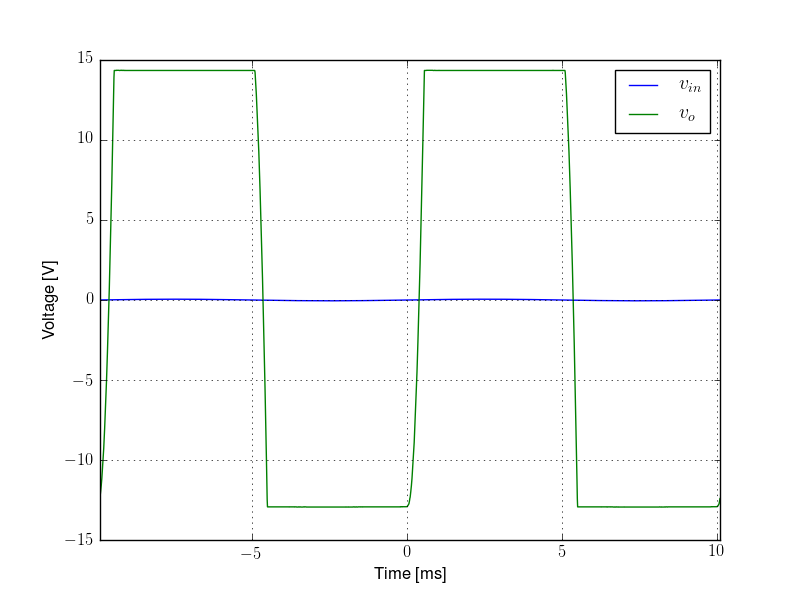
\includegraphics[width=.7\textwidth]{1/scope1.png}
\caption{Open loop configuration}
\end{figure}
In the open loop configuration we get an output (visible in figure 1.6) that has a maximum absolute value of $14.35\pm 0.16$\footnote{Error based on oscilloscope's 8 bit resolution} V and a minimum value of $-12.94\pm 0.16^1$ V. According to the ideal model we would expect the output to be infinite, as stated by the equation $v_o = A_{ol}(v_+-v_-)$ where $A_{ol}$ tends to infinity. In the physical case the output voltage is costrained by the saturation voltage that's determined by the voltage applied to the op-amp.
The minimum and maximum output values are different in modulus, due to the lack of symmetry between the \emph{npn} and \emph{pnp} trasistors in the final push-pull stage of the op-amp. 
\begin{figure}[H]
\centering
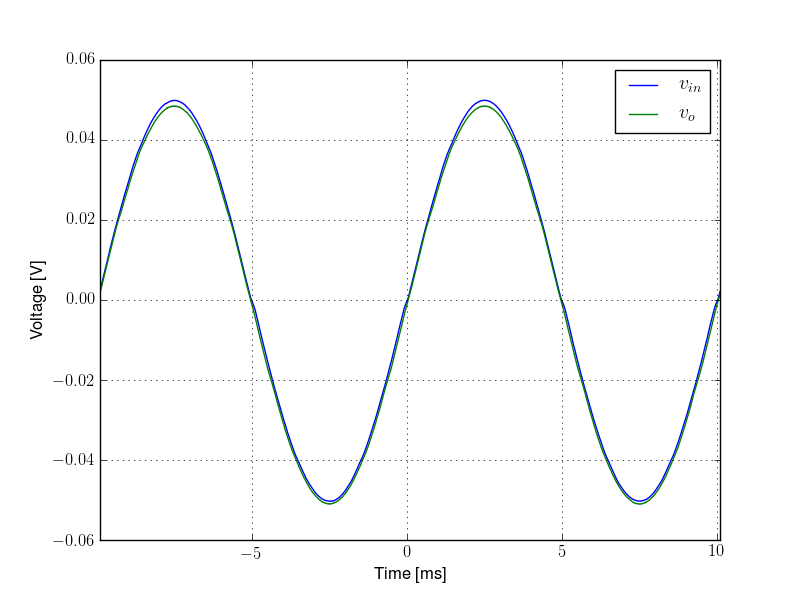
\includegraphics[width=.7\textwidth]{1/scope2.png}
\caption{Emitter follower}
\end{figure}
Regarding the emitter follower we expect, ideally, an output voltage equal to the input one. Actually we can see in the plot a small discrepancy between the two signals: that is probably determined by the op-amp's offset, as we can see a downward translation in the output, and also by some other non ideal features of the op-amp.
\begin{figure}[H]
\centering
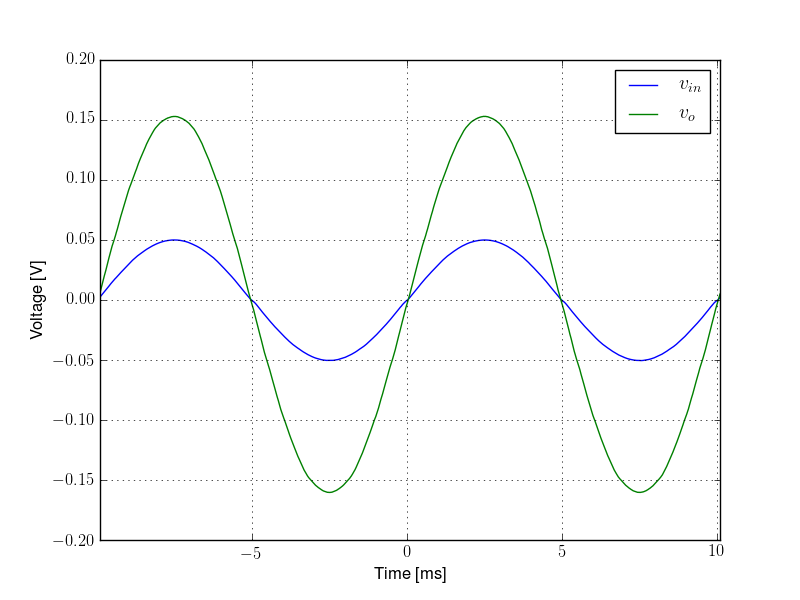
\includegraphics[width=.7\textwidth]{1/scope3.png}
\caption{Non-inverting amplifier}
\end{figure}
In the non-inverting amplifier configuration we expect the output voltage to be: $v_o = v_{in} (1 + \frac{R_2}{R_1})$. The theoretical value for the  peak-peak output voltage calculated using $R_1$, $R_2$ and $v_{in}$ is $320.3\pm 1.9$ mV. This prediction is not compatible with the output measured $313.4\pm 0.8$ mV of a $3.3 \sigma$ factor, probably because the op-amp is not ideal.
\begin{figure}[H]
\centering
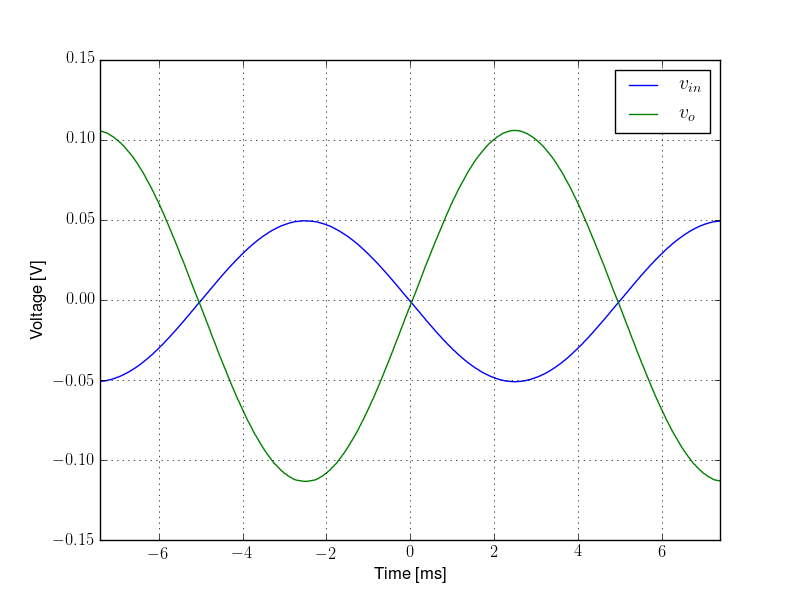
\includegraphics[width=.7\textwidth]{1/scope4.png}
\caption{Inverting amplifier}
\end{figure}
In the inverting amplifier the output should be : $v_o = - v_{in} \frac{R_2}{R_1}$. The pk-pk value of the output is $219.4\pm 0.8$ mV that is fully compatible with theoretical value $219.8\pm 1.9$ mV.
\begin{figure}[H]
\centering
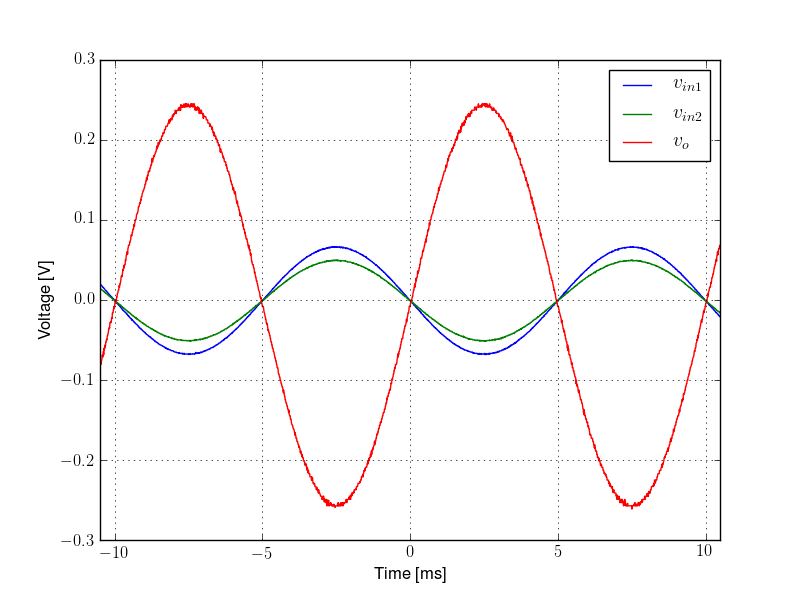
\includegraphics[width=.7\textwidth]{1/scope5.png}
\caption{Weighted summing circuit}
\end{figure}
In circuit 1.10 we used two different inputs for aquiring an output voltage: this configuration sums these signals $v_1 = 135.1\pm 0.8$ mV and $v_2 = 101.3\pm 0.8$ mV using the resistors $R_1$ and $R_3$ as weights, giving as output $v_o = - R_2 (\frac{v_1}{R_1} + \frac{v_2}{R_3})$, which gives a pk-pk value of $516.7\pm 2.7$ mV. The theory in this case is not compatible with the measurament $506\pm 0.8$ mV by a $3.8 \sigma$ factor, a little more than the previous result, but that's most likely caused by the unavoidable noise in the output.

\chapter{Let's get more confident with our little friend op-amp}
We designed a non-inverting amplifier with a variable gain using a trimmer. The second circuit designed was a summing amplifier with unitary gain. We built a current source generator of $1$ mA and tested it with various loads. We tested the efficacy of the emitter follower configuration in mismatching the source's impedence. At last we designed a differential amplifier with a predetermined gain.
\section{Materials}
\begin{itemize}
\item Operational amplifier uA741
\item Resistors and trimmers
\item Power supply RIGOL DP831A
\item Waveform generator RIGOL DG1032
\item Multimeter RIGOL DM3068
\item Oscilloscope RIGOL MS02102A
\item Two capacitance of nominal value of $100$nF
\end{itemize}
\section{Experiment setup}
In each circuit we powered the op-amp with a $\pm15$ V DC voltage and, in order to reduce possible noises, we added two 100nF capacitors connecting the op-amp's pins for the power supply with the ground. The input signal has a frequency of 100 Hz and a peak-peak voltage of 1V except for the differential amplifier. For every specific circuit we designed them as follow:
\begin{itemize}
\item Inverting amplifier: we placed a 10k$\Omega$ trimmer along the feedback branch in series to a resistor $R_f = 983.9 \pm 0.1 \Omega$. In order to have a minimal gain of 5, we used $R_{in} = 199.84\pm 0.03 \Omega$ as in figure \eqref{Non-inverting variable amplifier}.
\item Summing amplifier: caring for the simplest calculations, we used $R_1 = 1484.7 \pm 0.2 \Omega \simeq R_2= 1483.5\pm 0.2\Omega$ so the equation is $\displaystyle\frac{v_1+v_2}{2}\left(1+\frac{R_4}{R_3}\right)$. For obtaining the sum of the input in output, we had to choose $R_3 = R_4 = 1001.3 \pm 0.1 \Omega$. The inputs $v_1$ and $v_2$ are the same 100 Hz, 1 V peak-peak sine wave signal.

\begin{figure}[H]
\centering
\begin{minipage}{.5\textwidth}
  \centering
\begin{circuitikz}
\draw(0,0) node[op amp] (opamp) {}
	%(opamp.+) node[left] {$v_+$}
	(opamp.+) ++ (-.3,0) node[ground] {} -- (opamp.+) 
	(opamp.out) to[short] (1.8,0) node[right] {$v_o$}
	(opamp.down) ++(0,-.7) node[below] {$-v_{cc}$} -- (opamp.down)
	(opamp.up) ++ (0,.7) node[above] {$+v_{cc}$} -- (opamp.up)
	(opamp.down) ++ (0,-.25)to[C,/tikz/circuitikz/bipoles/length=1cm] (1,-.8)node[ground,rotate = 90,yshift = 1em] {}
	(opamp.up) ++ (0,.25)to[C,/tikz/circuitikz/bipoles/length=1cm] (1,.8)node[ground,rotate = 90,yshift = 1em] {};
	\draw(-4,-1) to[sV,l=$v_{in}$] (-4,.5) to[R=$R_{in}$] (-2,.5) to[short] (opamp.-);
	\draw(-4,-1) node[ground] {};
	
	\draw(-1.5,.5) to[short](-1.5,2.2) to[R=$R_f$](0,2.2) to[vR=$R_x$] (1.5,2.2)  to[short](1.5,0);
\end{circuitikz}
\caption{Inverting variable amplifier}\label{Non-inverting variable amplifier}
\end{minipage}%
\begin{minipage}{.5\textwidth}
  \centering
\begin{circuitikz}
\draw(0,0) node[op amp] (opamp) {}
	%(opamp.+) node[left] {$v_+$}
	%(opamp.+) ++ (-.3,0) node[ground] {} -- (opamp.+) 
	(opamp.out) to[short] (1.8,0) node[right] {$v_o$}
	(opamp.down) ++(0,-.7) node[below] {$-v_{cc}$} -- (opamp.down)
	(opamp.up) ++ (0,.7) node[above] {$+v_{cc}$} -- (opamp.up)
	(opamp.down) ++ (0,-.25)to[C,/tikz/circuitikz/bipoles/length=1cm] (1,-.8)node[ground,rotate = 90,yshift = 1em] {}
	(opamp.up) ++ (0,.25)to[C,/tikz/circuitikz/bipoles/length=1cm] (1,.8)node[ground,rotate = 90,yshift = 1em] {};
	\draw(-4,-.5)node[left]{$v_1$} to[R=$R_{1}$,o-] (-2,-.5) to[short] (opamp.+);
	\draw(-4,-1.5)node[left]{$v_2$} to[R=$R_{2}$,o-] (-2,-1.5) to[short] (-2,-.5);

	\draw(opamp.-) -- (-1.5,.5) to[short](-1.5,2.2) to[R=$R_4$](1.5,2.2) to[short](1.5,0);
	\draw(-1.5,2.2) to[R=$R_3$] (-4,2.2)node[ground] {};
\end{circuitikz}
\caption{Non-inverting summing amplifier, unitary gain}
\end{minipage}
\end{figure}
\item Emitter follower test: at first we built a circuit without the emitter follower using an input impedence of $R=100.2\pm 1\, \text{k}\Omega$ and a load of $R_L=19.8\pm 2\,\text{k}\Omega$.  Then we added the op-amp stage and compared the output measurements in the 2 different cases.
\begin{figure}[H]
\centering
\begin{minipage}{.5\textwidth}
  \centering
\begin{circuitikz}
\draw(0,0)node[ground]{} to[sV] (0,2) to[R=$R$,-o]node[right,xshift=.8em] {$v_o$} (2,2);
\draw(1.8,2) to[R=$R_L$](1.8,0)node[ground]{};
\end{circuitikz}
\caption{Test circuit without follower}
\end{minipage}%
\begin{minipage}{.5\textwidth}
  \centering
\begin{circuitikz}
\draw(0,0) node[op amp] (opamp) {}
	%(opamp.+) node[left] {$v_+$}
	(opamp.+) ++ (-.3,0) node[ground] {} -- (opamp.+) 
	(opamp.out) to[short,-o] (1.8,0) node[right] {$v_o$}
	(opamp.down) ++(0,-.7) node[below] {$-v_{cc}$} -- (opamp.down)
	(opamp.up) ++ (0,.7) node[above] {$+v_{cc}$} -- (opamp.up)
	(opamp.down) ++ (0,-.25)to[C,/tikz/circuitikz/bipoles/length=1cm] (1,-.8)node[ground,rotate = 90,yshift = 1em] {}
	(opamp.up) ++ (0,.25)to[C,/tikz/circuitikz/bipoles/length=1cm] (1,.8)node[ground,rotate = 90,yshift = 1em] {};
	\draw(-4,-1) to[sV,l=$v_{in}$] (-4,.5) to[R=$R$] (-2,.5) to[short] (opamp.-);
	\draw(-4,-1) node[ground] {};
	\draw(-1.5,.5) to[short](-1.5,2.2)to[short] (1.5,2.2)  to[short](1.5,0);
	\draw(1.6,0) to[R=$R_L$] (1.6,-2)node[ground]{};
\end{circuitikz}
\caption{Test circuit with follower}
\end{minipage}
\end{figure}

\item Current generator: the aim of this circuit is to generate a stable fixed current indipendent from the load. We generated a $1$ mA current using a DC voltage source of 5 V and a 4.9693 $\pm$ 0.7 k$\Omega$ resistor. The load was simulated with a trimmer. 
\item Differential amplifier: the full equation the circuit in figure \eqref{differential amplifier} is the following:
\[v_o = \frac{R_F}{R_1}\left[\frac{v_b}{1+R_f/Ry}\left(1+\frac{R_1}{R_f}\right)-v_a\right]\]
we first set to ground $v_b$, in this way we were able to set up the gain of the circuit (we chose it to be $A=2$ with $R_F =3\pm 0.2\, \text{k}\Omega$ (5\% error of nominalvalue)). After that we put the same signal of $v_a$ in $v_b$ with a resistor $R_f$ and a variable resistor $R_y$ made with $R_2$ in series with a trimmer. We managed with the trimmer to get the output as close to zero as possibile (Figure \eqref{Tuning_diff-amplifier}). This means in the equation $R_f/R_y = R_1/R_F$ so the new output is exaclty what we want $v_0 = A(v_b-v_a)$. For testing the amplifier we used $v_a= 5$ V DC and for $v_b$ a sine wave 1 V peak-peak 100 Hz with an offset of 5 V.
\end{itemize}

\begin{figure}[H]
\centering
\begin{minipage}{.5\textwidth}
  \centering
\begin{circuitikz}
\draw(0,0) node[op amp] (opamp) {}
	%(opamp.+) node[left] {$v_+$}
	(opamp.+) ++ (-.3,0) node[ground] {} -- (opamp.+) 
	(opamp.out) to[short] (1.8,0) node[right] {$v_o$}
	(opamp.down) ++(0,-.7) node[below] {$-v_{cc}$} -- (opamp.down)
	(opamp.up) ++ (0,.7) node[above] {$+v_{cc}$} -- (opamp.up)
	(opamp.down) ++ (0,-.25)to[C,/tikz/circuitikz/bipoles/length=1cm] (1,-.8)node[ground,rotate = 90,yshift = 1em] {}
	(opamp.up) ++ (0,.25)to[C,/tikz/circuitikz/bipoles/length=1cm] (1,.8)node[ground,rotate = 90,yshift = 1em] {};
	\draw(-4,-.8) to[battery1] (-4,.5) to[R=$R_{3}$] (-2,.5) to[short] (opamp.-);
	\draw(-4,-.5) node[ground] {};
	
	\draw(-1.5,.5) to[short](-1.5,2.2) to[vR=$R_x$] (1.7,2.2)to[myvoltmeter](1.7,0);
\end{circuitikz}
\caption{Current source generator}
\end{minipage}%
\begin{minipage}{.5\textwidth}
  \centering
\begin{circuitikz}
\draw(0,0) node[op amp] (opamp) {}
	%(opamp.+) node[left] {$v_+$}
	%(opamp.+) ++ (-.3,0) node[ground] {} -- (opamp.+) 
	(opamp.out) to[short] (1.8,0) node[right] {$v_o$}
	(opamp.down) ++(0,-.7) node[below] {$-v_{cc}$} -- (opamp.down)
	(opamp.up) ++ (0,.7) node[above] {$+v_{cc}$} -- (opamp.up)
	(opamp.down) ++ (0,-.25)to[C,/tikz/circuitikz/bipoles/length=1cm] (1,-.8)node[ground,rotate = 90,yshift = 1em] {}
	(opamp.up) ++ (0,.25)to[C,/tikz/circuitikz/bipoles/length=1cm] (1,.8)node[ground,rotate = 90,yshift = 1em] {};
	\draw(-4,-.5)node[left]{$v_B$} to[R=$R_{f}$,o-] (-2,-.5) to[short] (opamp.+);
	\draw((-2,-.5) to[vR=$R_{y}$] (-2,-2.5) node[ground]{};

	\draw(opamp.-) -- (-1.5,.5) to[short](-1.5,2.2) to[R=$R_F$](1.5,2.2) to[short](1.5,0);
	\draw(-1.5,2.2) to[R=$R_1$,-o] (-4,2.2)node[left] {$v_A$};
\end{circuitikz}
\caption{differential amplifier}\label{differential amplifier}
\end{minipage}
\end{figure}
\begin{figure}[H]
\centering
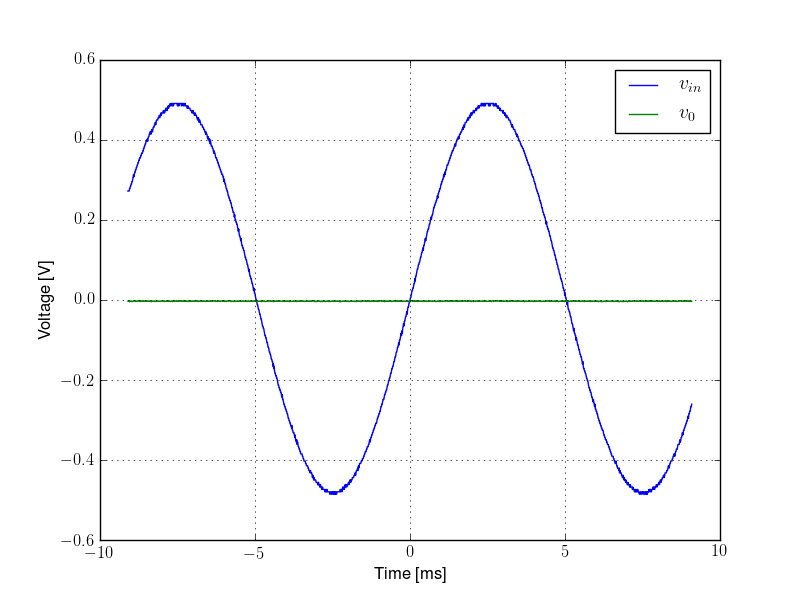
\includegraphics[width=.7\textwidth]{2/Tuning_diff-amplifier.png}
\caption{Calibration of the differential amplifier}\label{Tuning_diff-amplifier}
\end{figure}
\section{Data analysis}
\begin{figure}[H]
\centering
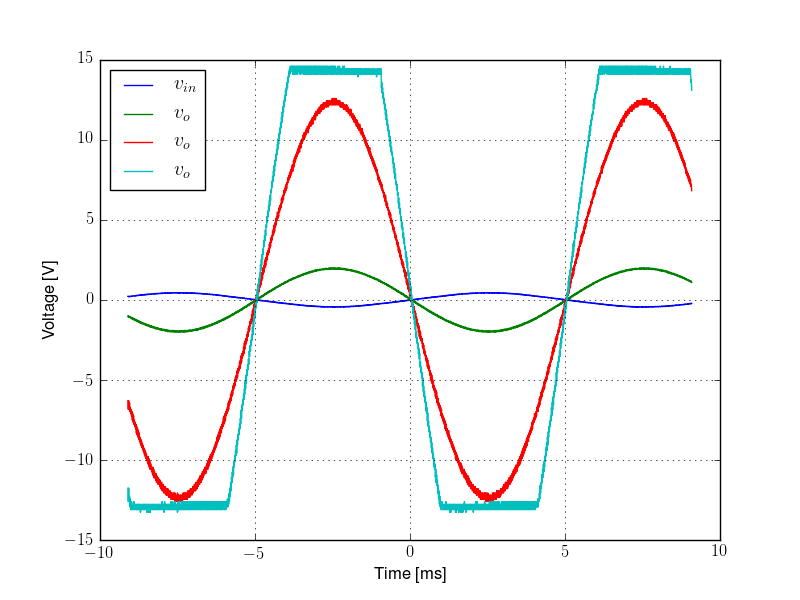
\includegraphics[width=.7\textwidth]{2/Variable_amplifier.png}
\caption{Variable amplifier}\label{Variableamplifier}
\end{figure}
In the inverting amplifier we used a trimmer in order to vary the gain, in fact the equation is:
\[v_{o} = -v_{in}\frac{R_f+R_x}{R_{in}}\]
so increasing $R_x$ cause the output to increase linearly. The output voltage is limited by the op-amps's power supply voltage, it cannot increase further and the signal goes flat, as we can see in figure \eqref{Variableamplifier} (light blue line), this behavior is called ``Clipping''. The graphic also shows a discrepance between the absolut value of maximum and minimum voltage during the clipping: this is due to the asimmetry between \emph{pnp} and \emph{npn} transistors in the op-amp's final stage.
\begin{figure}[H]
\centering
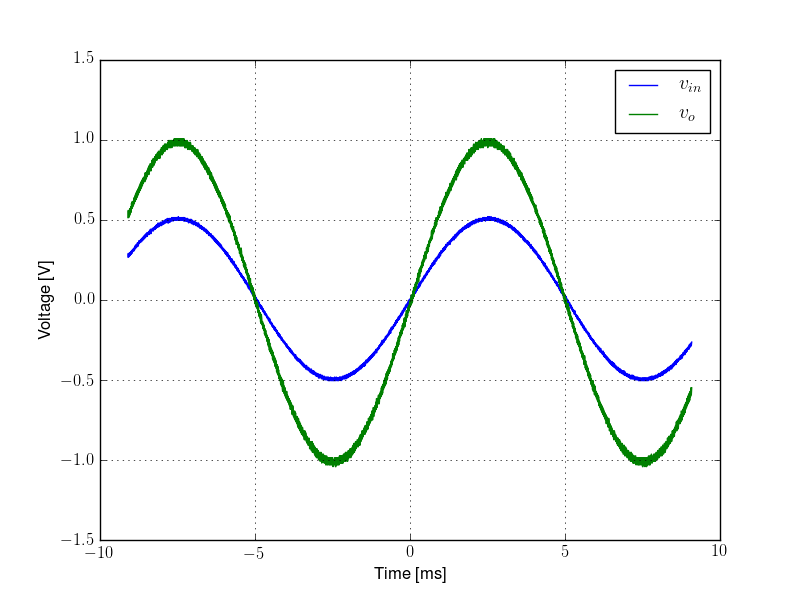
\includegraphics[width=.7\textwidth]{2/Weighted_amplifier.png}
\caption{Weighted summing amplifier}\label{Weighted_amplifier}
\end{figure}
In the non-inverting summing amplifier circuit we wanted the output to be the simple sum of the signals in entrance, that were identical: it means that the output signal must have double amplitude compared to the input one. The peak-peak voltage's theoretical expectation is $2.0496 \pm 0.0009$ V while the measured one is $2.032 \pm 0.001 $ V. The incompatibility probably is due to the op-amp's non-ideality.
\begin{figure}[H]
\centering
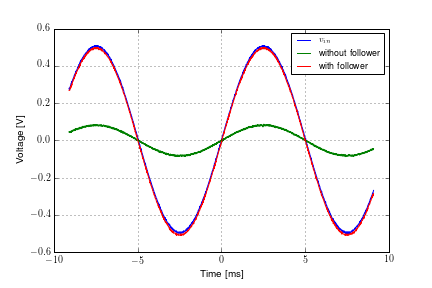
\includegraphics[width=.7\textwidth]{2/Emitter_follower_compared.png}
\caption{Emitter follower comparison}\label{Emitter_follower_compared}
\end{figure}
Let's now analyse the differences between circuits with and without follower stage. We can see in figure \eqref{Emitter_follower_compared} that using the follower we obtain a replicated signal while without it the signal is shrinked due to the input impedence, in fact the op-amp stage's purpose is the impedence mismatching.\\
\newline
In the current generator circuit we firstly measured the output current that was the expected one, than we observed the indipendency from the trimmer resistence of the current value.
\begin{figure}[H]
\centering
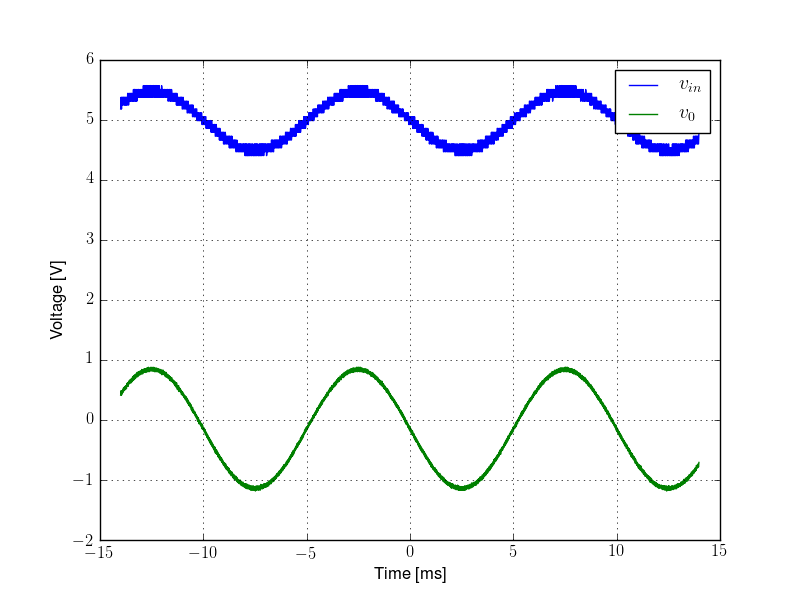
\includegraphics[width=.7\textwidth]{2/Differential_amplifier.png}
\caption{Differential amplifier}\label{Differential amplifier}
\end{figure}
In the differential amplifier circuit we measured an output cleared from the DC part present in the input, the output value was the AC part doubled compared to the input one. This is exactly how we expected the circuit to behave.

\chapter{Unfortunately the op-amp is not so ideal}
In this set of experiments we dealt with the problems of a real op-amp such as the offset $v_{os}$, the bias currents $i_{b+},i_{b-}$, the slew-rate, the maximum current output and the common gain $A_{cm}$: we measured all of these parameters. The offset was studied with 3 different circuits and then compensated with a trimmer in the configuration suggested by the op-amp's datasheet. The bias currents were measured in two ways, one for the bias current in the non inverting op-amp input and one for the inverting one. The other parameters were studied simply adjusting the input for the measurement's purpose.

\section{Materials}
\begin{itemize}
\item Operational amplifier uA741
\item Resistors, trimmers and capacitors
\item Power supply RIGOL DP831A
\item Waveform generator RIGOL DG1032
\item Multimeter RIGOL DM3068
\item Oscilloscope RIGOL MS02102A
\end{itemize}
\begin{table}[H]
\centering
\begin{tabular}{ |p{3cm}||p{3cm}|p{3cm}| }
 \hline
 \multicolumn{3}{|c|}{List of resistors used} \\
 \hline
 Resistor name & Value [$\Omega$] & Uncertainty [$\Omega$]\\
 \hline
 R$_{\text{M}\Omega}$   & 982.0 $\times$ 10$^3$ & 0.1 $\times$ 10$^3$  \\
 R$_{100\text{k}\Omega}$& 99.22 $\times$ 10$^3$ & 0.01 $\times$ 10$^3$ \\
 R$_{10\text{k}\Omega}$ &   9906.2            & 1.2         \\
 R$_{\text{k}\Omega}$   &  1001.4             & 0.1         \\
 R$_{10\Omega}$         &  9.963              & 0.01        \\
 R$_{10\text{k}\Omega}^*$ &  9926.4             & 1.2         \\
 R$_{10\Omega}^*$       &10.00                & 0.01        \\ 
 \hline
\end{tabular}
\end{table}

\section{Experiment setup}
In all the circuits we placed on the power supply's pins two capacitors each, one with high capacitace (nominal value 470 $\pm$ 23 nF) and one with low capacitance (10.0 $\pm$ 0.5 nF). These were used for suppressing the high-frequency noise and contrasting the effect of any eventual change in the power supply voltage, that could move the offset voltage.
\begin{figure}[H]
\centering
\begin{minipage}{.32\textwidth}
  \centering
  \begin{circuitikz}
 	\draw(0,0) node[op amp] (opamp) {}
	%(opamp.+) node[left] {$v_+$}
	(opamp.-) ++ (-.3,0) -- (opamp.-) 
	(opamp.-) ++ (-.3,0) -- (-1.5,1.8) -- (1.6,1.8) -- (1.6,0)
	(opamp.out) to [short,-o](1.8,0) node[right] {$v_o$}
	(opamp.up) ++(0,.5) node[above] {$+v_{cc}$} -- (opamp.up)
	(opamp.down) ++ (0,-.5) node[below] {$-v_{cc}$} -- (opamp.down)
	(opamp.down) ++ (0,-.25)to[C,/tikz/circuitikz/bipoles/length=1cm] (1,-.8)node[ground,rotate = 90,yshift = 1em] {}
	(opamp.up) ++ (0,.25)to[C,/tikz/circuitikz/bipoles/length=1cm] (1,.8)node[ground,rotate = 90,yshift = 1em] {};
	\draw(opamp.+) ++ (-.3,0)node[ground] {} -- (opamp.+);
	\end{circuitikz}
\caption{Offset voltage's direct measure}\label{offset direct}
\end{minipage}%
\begin{minipage}{.32\textwidth}
  \centering
  \begin{circuitikz}
\draw(0,0) node[op amp] (opamp) {}
	%(opamp.+) node[left] {$v_+$}
	(opamp.+) ++ (-.3,0) node[ground] {} -- (opamp.+) 
	(opamp.out) to [short,-o](1.8,0) node[right] {$v_o$}
	(opamp.down) ++(0,-.5) node[below] {$-v_{cc}$} -- (opamp.down)
	(opamp.up) ++ (0,.5) node[above] {$+v_{cc}$} -- (opamp.up)
	(opamp.down) ++ (0,-.25)to[C,/tikz/circuitikz/bipoles/length=1cm] (1,-.8)node[ground,rotate = 90,yshift = 1em] {}
	(opamp.up) ++ (0,.25)to[C,/tikz/circuitikz/bipoles/length=1cm] (1,.8)node[ground,rotate = 90,yshift = 1em] {};
	\draw(-3.1,.5) to[R,l=R$_{10\Omega}$] (-1.5,.5) to[short] (opamp.-);
	\draw(-3.1,.5) node[ground] {};
	\draw(-1.5,.5) to[short](-1.5,2.2) to[R,l=R$_{10\text{k}\Omega}$](1.5,2.2) to[short](1.5,0);
\end{circuitikz}
\caption{Offset voltage's direct measure with gain}\label{offset amp}
\end{minipage}%
\begin{minipage}{.32\textwidth}
  \centering
\begin{circuitikz}
\draw(0,0) node[op amp] (opamp) {}
	%(opamp.+) node[left] {$v_+$}
	%(opamp.+) ++ (-.3,0) node[ground] {} -- (opamp.+) 
	(opamp.out) to [short,-o](1.8,0) node[right] {$v_o$}
	(opamp.down) ++(0,-.5) node[below] {$-v_{cc}$} -- (opamp.down)
	(opamp.up) ++ (0,.5) node[above] {$+v_{cc}$} -- (opamp.up)
	(opamp.down) ++ (0,-.25)to[C,/tikz/circuitikz/bipoles/length=1cm] (1,-.8)node[ground,rotate = 90,yshift = 1em] {}
	(opamp.up) ++ (0,.25)to[C,/tikz/circuitikz/bipoles/length=1cm] (1,.8)node[ground,rotate = 90,yshift = 1em] {};
	\draw(-3,.5) to[R,l=R$_{10\Omega}$] (-1.5,.5) to[short] (opamp.-);
	\draw(-3,.5) node[ground] {};
	\draw(-1.5,.5) to[short](-1.5,2.2) to[R,l=R$_{10\text{k}\Omega}$](1.5,2.2) to[short](1.5,0);
	
	\draw(opamp.+) to[short](-1.7,-.5)to[short](-1.7,-1) to[short](-2.1,-1) to[R,l_=R$^*_{10\text{k}\Omega}$](-2.1,-3)to[short](-1.7,-3)node[ground]{};
	\draw(-1.7,-1)to[short](-1.3,-1)to[R,l=R$^*_{10\Omega}$](-1.3,-3)to[short](-1.7,-3);
\end{circuitikz}
\caption{Offset voltage's direct measure with gain and bias current correction}\label{offset amp corrected}
\end{minipage}
\end{figure}
In the first circuit we measured $v_{os}$ directly by using the multimeter on the output voltage.
We used the second circuit drawn to amplify $v_{os}$, we measured the amplified signal.\\
The third circuit is identical to the second except for the added resistors in parallel that connect the non inverting pin to the ground: this was done for removing the bias current influence from the measurament according to the hypothesis that these currents are approximately equal. For this reason these added resistors need to have toghether the same resistance of the parallel between the $R_{10 \Omega}$ and $R_{10 k\Omega}$ used before.\ Exploiting this last circuit we removed $v_{os}$ by using a trimmer between op-amp pins 1 and 5, paying attention to connect the central trimmer pin to the negative power supply voltage (according to the uA741 datasheet): we tried to make the output as close to 0 as possible (we used no input voltage in these steps).
\begin{figure}[H]
\centering
\begin{minipage}{.5\textwidth}
  \centering
\begin{circuitikz}
\draw(0,0) node[op amp] (opamp) {}
	%(opamp.+) node[left] {$v_+$}
	%(opamp.+) ++ (-.3,0) node[ground] {} -- (opamp.+) 
	(opamp.out) to [short,-o](1.8,0) node[right] {$v_o$}
	%(opamp.down) ++(0,-.5) node[below] {$-v_{cc}$} -- (opamp.down)
	(opamp.up) ++ (0,.5) node[above] {$+v_{cc}$} -- (opamp.up)
	(opamp.down) ++ (0,-.25)to[C,/tikz/circuitikz/bipoles/length=1cm] (1,-.8)node[ground,rotate = 90,yshift = 1em] {}
	(opamp.up) ++ (0,.25)to[C,/tikz/circuitikz/bipoles/length=1cm] (1,.8)node[ground,rotate = 90,yshift = 1em] {};
	\draw(-3.5,.5) to[R,l=R$_{\text{k}\Omega}$] (-1.5,.5) to[short] (opamp.-);
	\draw(-3.5,.5) node[ground] {};
	\draw(-1.5,.5) to[short](-1.5,2.2) to[R,l=R$_{100\text{k}\Omega}$](1.5,2.2) to[short](1.5,0);
	\draw(opamp.+) to[short](-1.2,-.5)to[R,l_=R$_{\text{M}\Omega}$](-1.2,-2.5)node[ground]{};
	\draw(opamp.down) ++ (-.45,-.25)to[short](-0.53,-2)to[R](1.53,-2);
	\draw(opamp.down) ++ (.6,.36) to[short](.515,-.35) to[short](1.53,-.35) to[short](1.53,-2);	
	\draw(opamp.down) to [short](-.085,-1.3)to[short](.42,-1.3);	
	\draw(-.085,-1.3) to[short](-.085,-1.45)node[below]{\scriptsize$-v_{cc}$};
	\draw[-stealth](.415,-1.3) -- (.415,-1.76);
\end{circuitikz}
\caption{Positive bias current measure}\label{current positive}
\end{minipage}%
\begin{minipage}{.5\textwidth}
\centering
\begin{circuitikz}
\draw(0,0) node[op amp] (opamp) {}
	%(opamp.+) node[left] {$v_+$}
	(opamp.+) ++ (-.3,0) node[ground] {} -- (opamp.+) 
	(opamp.out) to [short,-o](1.8,0) node[right] {$v_o$}
	%(opamp.down) ++(0,-.5) node[below] {$-v_{cc}$} -- (opamp.down)
	(opamp.up) ++ (0,.5) node[above] {$+v_{cc}$} -- (opamp.up)
	(opamp.down) ++ (0,-.25)to[C,/tikz/circuitikz/bipoles/length=1cm] (1,-.8)node[ground,rotate = 90,yshift = 1em] {}
	(opamp.up) ++ (0,.25)to[C,/tikz/circuitikz/bipoles/length=1cm] (1,.8)node[ground,rotate = 90,yshift = 1em] {};
	\draw(-5,.49) to[R,l=R$_{\text{k}\Omega}$] (-3,.49) to[R,l=R$_{100\text{k}\Omega}$](-1,.49);%to[short](opamp.-);
	\draw(-5,.49) node[ground] {};
	\draw(-3,.49) to[short](-3,2.2) to[R,l=R$_{\text{M}\Omega}$](1.5,2.2) to[short](1.5,0);
	%\draw(opamp.+) to[short](-1.2,-.5)node[ground]{};
	\draw(opamp.down) ++ (-.45,-.25)to[short](-0.53,-2)to[R](1.53,-2);
	\draw(opamp.down) ++ (.6,.36) to[short](.515,-.35) to[short](1.53,-.35) to[short](1.53,-2);	
	\draw(opamp.down) to [short](-.085,-1.3)to[short](.42,-1.3);
	\draw(-.085,-1.3) to[short](-.085,-1.45)node[below]{\scriptsize$-v_{cc}$};
	\draw[-stealth](.415,-1.3) -- (.415,-1.76);
\end{circuitikz}
\caption{Negative bias current measure}\label{current negative}
\end{minipage}
\end{figure}
The fourth circuit and the fifth are used for measuring the bias currents indirectly basing on how the two currents are related to the output: we use a great resistance ($R_{M\Omega}$) in order to make relevant to a voltage measurement only one bias current with respect to the other.\\
The sixth circuit was used for measuring the maximum current that the op-amp can erogate. In this configuration the oscilloscope's internal resitor was set to $50 \Omega$.\\
\begin{figure}[H]
\centering
\begin{minipage}{.5\textwidth}
\centering
\begin{circuitikz}
 	\draw(0,0) node[op amp] (opamp) {}
	%(opamp.+) node[left] {$v_+$}
	(opamp.-) ++ (-.3,0) -- (opamp.-) 
	(opamp.-) ++ (-.3,0) -- (-1.5,1.8) -- (1.6,1.8) -- (1.6,0)
	(opamp.out) to [short](2.5,0)to[myvoltmeter,l=Oscilloscope $50\ohm$](2.5,-1.5)node[ground]{}
	(opamp.up) ++(0,.5) node[above] {$+v_{cc}$} -- (opamp.up)
	(opamp.down) ++ (0,-.25)to[C,/tikz/circuitikz/bipoles/length=1cm] (1,-.8)node[ground,rotate = 90,yshift = 1em] {}
	(opamp.up) ++ (0,.25)to[C,/tikz/circuitikz/bipoles/length=1cm] (1,.8)node[ground,rotate = 90,yshift = 1em] {};
	%\draw(opamp.+) ++ (-.3,0)node[ground] {} -- (opamp.+);
	\draw(opamp.down) ++ (-.45,-.25)to[short](-0.53,-2)to[R](1.53,-2);
	\draw(opamp.down) ++ (.6,.36) to[short](.515,-.35) to[short](1.53,-.35) to[short](1.53,-2);
	\draw(opamp.down) to [short](-.085,-1.3)to[short](.42,-1.3);
	\draw(-.085,-1.3) to[short](-.085,-1.45)node[below]{\scriptsize$-v_{cc}$};
	\draw[-stealth](.415,-1.3) -- (.415,-1.76);
	\draw(-2,-2)node[ground]{}to[tV](-2,-.5) -- (opamp.+);
	\draw(2.5,0)to[short,-o](2.8,0)node[right] {$v_o$};
	\end{circuitikz}
	\caption{Max current measure}\label{max current}
\end{minipage}%
\begin{minipage}{.5\textwidth}
\centering
\begin{circuitikz}
 	\draw(0,0) node[op amp] (opamp) {}
	%(opamp.+) node[left] {$v_+$}
	(opamp.-) ++ (-.3,0) -- (opamp.-) 
	(opamp.-) ++ (-.3,0) -- (-1.5,1.8) -- (1.6,1.8) -- (1.6,0)
	(opamp.out) to [short](2.5,0)to[short](2.5,-.3)to[short](2.2,-.3)to[C](2.2,-1.8)to[short](2.5,-1.8)node[ground]{}
	(opamp.up) ++(0,.5) node[above] {$+v_{cc}$} -- (opamp.up)
	(opamp.down) ++ (0,-.25)to[C,/tikz/circuitikz/bipoles/length=1cm] (1,-.8)node[ground,rotate = 90,yshift = 1em] {}
	(opamp.up) ++ (0,.25)to[C,/tikz/circuitikz/bipoles/length=1cm] (1,.8)node[ground,rotate = 90,yshift = 1em] {};
	%\draw(opamp.+) ++ (-.3,0)node[ground] {} -- (opamp.+);
	\draw(opamp.down) ++ (-.45,-.25)to[short](-0.53,-2)to[R](1.53,-2);
	\draw(opamp.down) ++ (.6,.36) to[short](.515,-.35) to[short](1.53,-.35) to[short](1.53,-2);
	\draw(opamp.down) to [short](-.085,-1.3)to[short](.42,-1.3);
	\draw(-.085,-1.3) to[short](-.085,-1.45)node[below]{\scriptsize$-v_{cc}$};
	\draw[-stealth](.415,-1.3) -- (.415,-1.76);
	\draw(-2,-2)node[ground]{}to[sqV](-2,-.5) -- (opamp.+);
	\draw(2.5,0)to[short,-o](2.8,0)node[right] {$v_o$};
	\draw(2.5,-.3)to[short](3,-.3)to[R](3,-1.8)to[short](2.5,-1.8);
	\end{circuitikz}
	\caption{Slew rate}\label{slew rate}
\end{minipage}
\end{figure}
With the seventh circuit we measured the slew rate: the load capacitor used was 1 $\pm$ 0.05 nF, the resistor 2 $\pm$ 0.1 k$\Omega$ and the input used a 0-10 V square wave, that allowed us to aquire the image of the raising output.\\
Finally, the last circuit allowed us to measure the common gain by using the differential amplifier with the same 2V peak-peak sine signal at 100 Hz as the two inputs.\\
\begin{figure}[H]
\centering
\begin{circuitikz}
\draw(0,0) node[op amp] (opamp) {}
	%(opamp.+) node[left] {$v_+$}
	%(opamp.+) ++ (-.3,0) node[ground] {} -- (opamp.+) 
	(opamp.out) to [short,-o](1.8,0) node[right] {$v_o$}
	(opamp.up) ++ (0,.5) node[above] {$+v_{cc}$} -- (opamp.up)
	(opamp.down) ++ (0,-.25)to[C,/tikz/circuitikz/bipoles/length=1cm] (1,-.8)node[ground,rotate = 90,yshift = 1em] {}
	(opamp.up) ++ (0,.25)to[C,/tikz/circuitikz/bipoles/length=1cm] (1,.8)node[ground,rotate = 90,yshift = 1em] {};
	\draw(-3.5,.5) to[R=$R_1$] (-1.5,.5) to[short] (opamp.-);
	\draw(-3.5,.5) to[short](-3.5,-.5);
	\draw(-1.5,.5) to[short](-1.5,2.2) to[R=$R_f$](1.5,2.2) to[short](1.5,0);
	\draw(-3.5,-.5) to[R=$R_1||R_f$] (-1.5,-.5) to[short] (opamp.+);
	\draw(-3.5,-.5) to[sV](-3.5,-2)node[ground]{};
	\draw(opamp.down) ++ (-.45,-.25)to[short](-0.53,-2)to[R](1.53,-2);
	\draw(opamp.down) ++ (.6,.36) to[short](.515,-.35) to[short](1.53,-.35) to[short](1.53,-2);
	\draw(opamp.down) to [short](-.085,-1.3)to[short](.42,-1.3);
	\draw(-.085,-1.3) to[short](-.085,-1.45)node[below]{\scriptsize$-v_{cc}$};
	\draw[-stealth](.415,-1.3) -- (.415,-1.76);
\end{circuitikz}
\caption{Common Gain}\label{common gain}
\end{figure}

\section{Data analysis}
In the emitter follower \eqref{offset direct} the output measured is $-1.484 \pm 0.005$ mV. Being such a small output we expect to have problems with parassite impedance and other forms of noise, that's why we don't consider this value too reliable. It however gives us an order of magnitude that matches the op-amp datasheet, according to which the absolute typical values are from 1 mV to 5 mV.\\
In the amplifier \eqref{offset amp} we can find $v_{os}$ resolving
\[v_{os} = \frac{v_{o}}{1 + \frac{R_{10\text{k}\Omega}}{R_{10\Omega}}}\]
From the calculation we get $v_{os} = -1.333 \pm 0.001$ mV, which has the same order of magnitude and sign of the previous result.\\
Then, as stated in the experimental setup, we corrected the circuit \eqref{offset amp corrected} for compensating the bias currents effect. With the same formula used for the previous amplifier we got an offset voltage of $1.307 \pm 0.001$ mV.\\
At this point we compensated the offset through the use of a trimmer (see experimental setup).\\
Regarding the fourth circuit \eqref{current positive}, we calculated the current flowing in the non invertent pin by using $$i_{b+} = -\frac{v_{o}}{R_{\text{M}\Omega} (1 + \frac{R_{100\text{k}\Omega}}{R_{1\text{k}\Omega}})}$$ The value calculated is $-39.042 \pm 0.009$ nA.\\
The fifth circuit \eqref{current negative} instead leads to the calculation of the current flowing in the invertent pin by using 
\[i_{b-} = \frac{v_{o}}{R_{100\text{k}\Omega}} \frac{R_{\text{k}\Omega}}{R_{\text{M}\Omega}}\]
we obtain the value $-39.724 \pm 0.009$ nA. Now we can compute the bias current $i_b = \frac{|i_{b-}| + |i_{b+}|}{2} = 39.383 \pm 0.006$ nA and the offset current $i_o = ||i_{b-}| - |i_{b+}|| = 0.68 \pm 0.01$ nA.\\
$i_b$ is less than 100 nA and near the typical value of 10 nA, as the datasheet states, but the offset current is a bit low being around a third of the typical value 2 nA.\\
\begin{figure}[H]
\centering
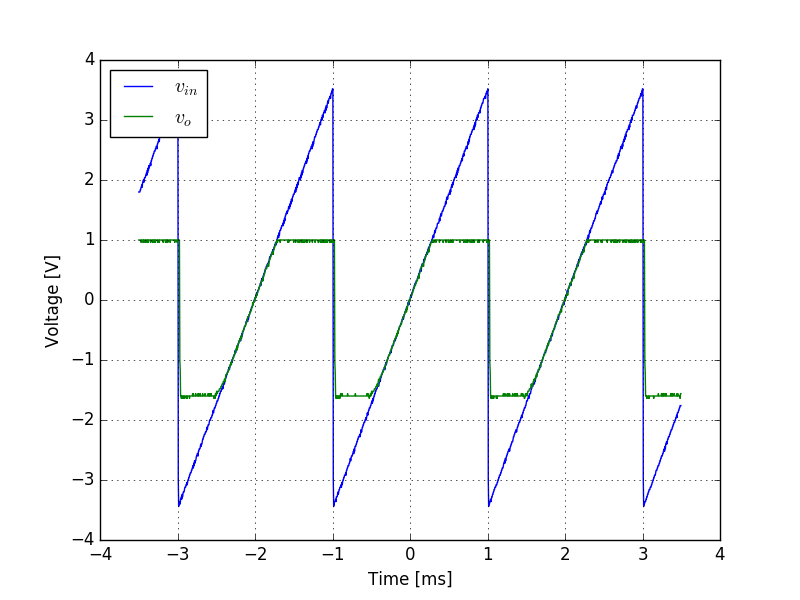
\includegraphics[width=.6\textwidth]{3/Maximum_current_erogated.png}
\caption{Saturated output caused by the maximum current erogated}
\end{figure}
In the sixth circuit \eqref{max current} we calculated the maximum current erogated by computing the maximum/minimum output voltage over the resistance in the oscilloscope. In the plot it is visible the different absolute value of the maximum and minimum output voltage, that's probably because the op-amp isn't perfectly symmetric in the packaging. So we chose to calculate two different maximum currents: $i_{max} = 0.0201 \pm 0.0001$ A (when the output was positive) and $i_{min} = -0.0328 \pm 0.0001$ (when the output was negative).
\begin{figure}[H]
\centering
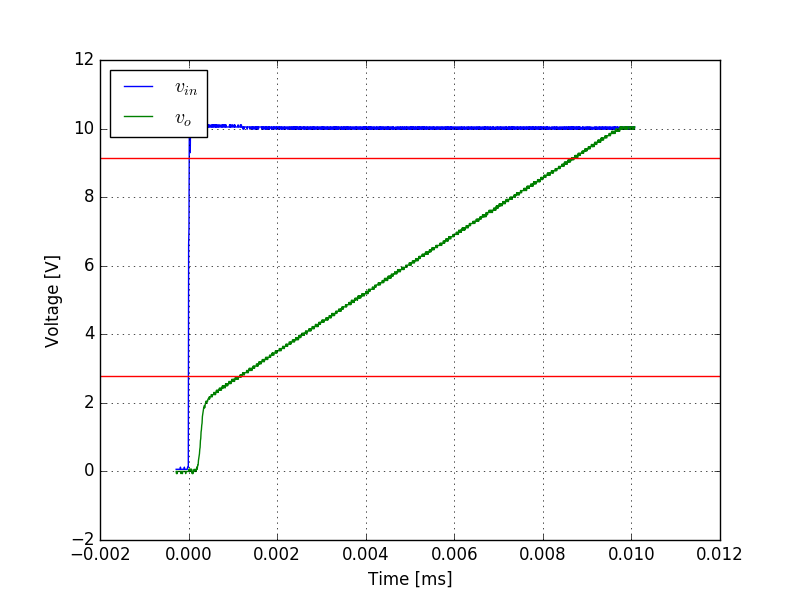
\includegraphics[width=.6\textwidth]{3/Slew_Ratio.png}
\caption{Output adjustment after an input change. Red lines are 10\% and 90\% of the output}
\end{figure}
In the seventh circuit \eqref{slew rate} we find that the slew rate ($\frac{\Delta V}{\Delta t}$) of the op-amp used is $0.8332 \pm 0.0026 \frac{\text{V}}{\mu s}$, which is bigger than the typical value $0.5 \frac{\text{V}}{\mu s}$. One possible explanation of this would be that the slew rate depends on the amplitude of the signal: in our experiment the voltage was 50 times larger than the test shown in the datasheet, otherwise we have to conclude that our op-amp, has some difects that cause a larger slew rate.
\begin{figure}[H]
\centering
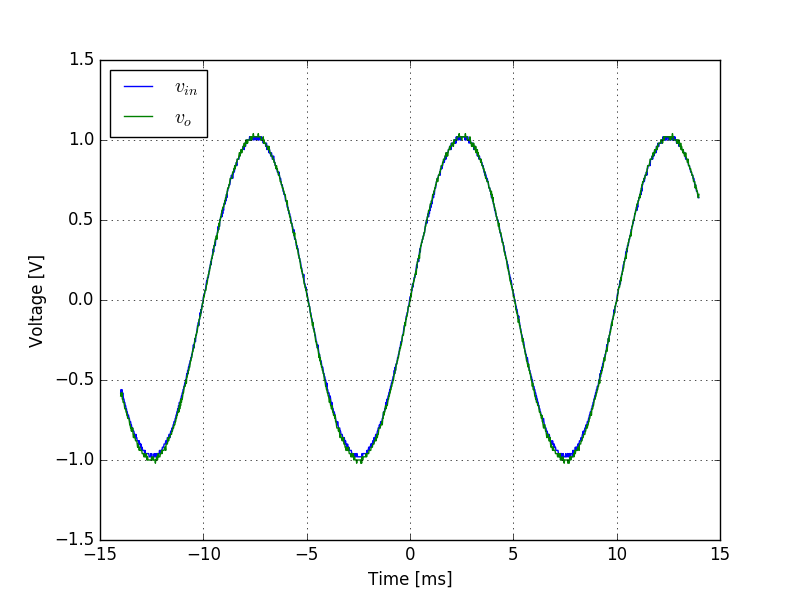
\includegraphics[width=.7\textwidth]{3/Amplification_in_common_mode.png}
\caption{Common gain measurement}
\end{figure}
With the last circuit \eqref{common gain} we measured the common gain of our op-amp by solving
\[A_{CM} = \frac{2 v_{o}}{v_{in1} + v_{in2}} = \frac{v_o}{v_{in}}\]
which gave us a unitary gain, $1.01 \pm 0.04 $, as it is evident in the plot. In an ideal situation this parameter should have been zero, in fact the value is pretty low: being the differential gain order of $10^5$ at low frequencies, we have a CMRR of 100 db that is quite high, this allows us to neglect the common gain most of the times.

\chapter{Gain in function of the frequency}
In a real op-amp the open loop gain ($A_{ol}$) is a function of the input frequency. In this experience we explored systematically this behaviour using 2 different circuits, one for the lower frequencies and the other for the higher ones. After this study we built a non inverting amplifier with $\approx 10$ and $\approx 100$ gain for measuring its bandwidth.

\section{Materials}
\begin{itemize}
\item Operational amplifier uA741
\item Resistors, trimmers, capacitors
\item Power supply RIGOL DP831A
\item Waveform generator RIGOL DG1032
\item Multimeter RIGOL DM3068
\item Oscilloscope RIGOL MS02102A
\end{itemize}
The resistor chosen were $R_1, R_2, R_3 = 10\text{k} \Omega$, $R_4 = 10 \Omega$, $R_5 = 100 \Omega, R_6 = 1\text{k}\Omega$ with an error of $5\%$ of the value.

\section{Experimental setup}
\begin{figure}[H]
\centering
\begin{minipage}{.5\textwidth}
  \centering
\begin{circuitikz}
\draw(0,0) node[op amp] (opamp) {}
	%(opamp.+) node[left] {$v_+$}
	(opamp.+) to[short] (-1.5,-.49)to[short](-1.5,-1.5)to[short](-2.5,-1.5)
	(opamp.out) to [short,-o](1.8,0) node[right] {$v_o$}
	(opamp.down) ++(0,-.5) node[below] {$-v_{cc}$} -- (opamp.down)
	(opamp.up) ++ (0,.5) node[above] {$+v_{cc}$} -- (opamp.up)
	(opamp.down) ++ (0,-.25)to[C,/tikz/circuitikz/bipoles/length=1cm] (1,-.8)node[ground,rotate = 90,yshift = 1em] {}
	(opamp.up) ++ (0,.25)to[C,/tikz/circuitikz/bipoles/length=1cm] (1,.8)node[ground,rotate = 90,yshift = 1em] {};
	\draw(opamp.-) to[short](-2.5,.49) to[R=$R_3$,-*](-2.5,2.2)node[above]{$v_a$} to[R,l=$R_2$](1.5,2.2) to[short](1.5,0);
	\draw(-2.5,.49)to[R,l_=$R_4$](-2.5,-1.5) node[ground]{};
	\draw(-4.5,.49)node[ground]{}to[sV](-4.5,2.2) to[R = $R_1$](-2.5,2.2);
\end{circuitikz}
\caption{$A_{ol}$ measure low frequencies}
\end{minipage}%
\begin{minipage}{.5\textwidth}
\begin{circuitikz}
\draw(0,0) node[op amp] (opamp) {}
	%(opamp.+) node[left] {$v_+$}
	(opamp.+) ++ (-.3,0) node[ground] {} -- (opamp.+) 
	(opamp.out) to [short,-o](1.8,0) node[right] {$v_o$}
	(opamp.down) ++(0,-.5) node[below] {$-v_{cc}$} -- (opamp.down)
	(opamp.up) ++ (0,.5) node[above] {$+v_{cc}$} -- (opamp.up)
	(opamp.down) ++ (0,-.25)to[C,/tikz/circuitikz/bipoles/length=1cm] (1,-.8)node[ground,rotate = 90,yshift = 1em] {}
	(opamp.up) ++ (0,.25)to[C,/tikz/circuitikz/bipoles/length=1cm] (1,.8)node[ground,rotate = 90,yshift = 1em] {};
	\draw(opamp.-) to[short](-2.5,.49) to[short,-*](-2.5,2.2)node[above]{$v_a$} to[R,l=$R_2$](1.5,2.2) to[short](1.5,0);
	\draw(-4.5,.49)node[ground]{}to[sV](-4.5,2.2) to[R,l=$R_1$](-2.5,2.2);
\end{circuitikz}
\caption{$A_{ol}$ measure high frequencies}
\end{minipage}
\end{figure}
In this experience we took the measurament in all circuits by changing the frequency of the input, that was a  sine wave signal 1 V peak-peak. The voltage chosen is not important, because we are interested in the ratio between the amplitude of the output and the input signals.\\
The first circuit was used for calculating the gain in the open loop configuration ($A_{ol}$) at low frequencies by measuring $v_a$ and $v_{o}$. This circuit was chosen for low freqencies instead of the second one, because the gain is too high for us to acquire directly the voltage difference between the two input pins. 
We didn't measure at frequencies lower than 30 Hz because the noise didn't allow us to make a reliable estimate of the two signals amplitude.\\
In the second circuit we measured $v_{o}$ and	 the voltage of the non inverting pin $v_a$. The frequencies measured went from 10 kHz to 200 kHz, because with high frequencies the absulute value of $A_{ol}$ is low enough.\\
In the last two circuits we built a non inverting amplifier (with a compensated offset) with a closed loop gain of 100 and 10, in order to verify the passing bandwidth.
\begin{figure}[H]
  \centering
  \begin{circuitikz}
 \draw(0,0) node[op amp,yscale=-1] (opamp) {}
%(opamp.+) node[left] {$v_+$}
(opamp.-) ++ (-.3,0) -- (opamp.-) 
(opamp.-) ++ (-.3,0) to[R,l_=$R_4$] (-3,-0.5) to (-3,-1) node[ground]{}
(opamp.-) ++ (-.3,0) -- (-1.5,-1.8) to[R,l_=$R_5$] (1,-1.8) -- (1,0)
(opamp.out) node[right] {$v_o$}
(opamp.up) ++(0,-.5) node[below] {$-v_{cc}$} -- (opamp.up)
(opamp.down) ++ (0,.5) node[above] {$+v_{cc}$} -- (opamp.down);
\draw(-4,-1) to[sV,l=$v_{in}$] (-4,.5) to[short] (opamp.+);
\draw(-4,-1) node[ground] {};
\end{circuitikz}
\caption{Non inverting amplifier}
\end{figure}

\section{Data Analysis}
\begin{figure}[H]
\centering
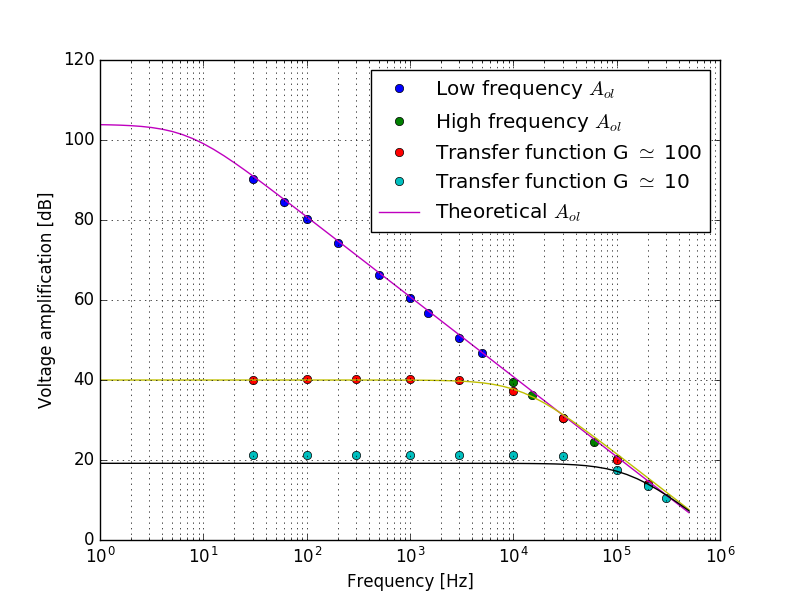
\includegraphics[width=.7\textwidth]{4/decibel.png}
\caption{Gain as a function of the frequency}
\end{figure}
Using the first circuit we can estimate from the formula $A_{ol} = - \frac{v_{o}}{v_a} \frac{R_3 + R_4}{R_4}$.
The same can be done with the second circuit, but this time the formula comes to be $A_{ol} = - \frac{v_{o}}{v_a}$. \\
We can see from the plot that the data appears to be on a straight line and it is also visible that this line is compatible with the values in the datasheet (the continuous line).
We can  however compute the theoretical open loop gain with: $$A_{ol}^{teo}(f) = \frac{A}{1 + j\frac{f}{f_0}}$$ where $f_0 = 8$ Hz is a parameter available in the datasheet and  $A = 1.5 \times 10^5$ was obtained with the best fit, $j$ is the immaginary unit and $f$ is the frequency. We can see from the plot that our data is consistent with the theory and the datasheet.\\
Regarding the last two circuit we plotted $H = \frac{v_{o}}{v_{in}}$ (the dots in the graph, experimental values), while the theoretical curve has been obtained thanks to the following formula:
\[H(f) = \frac{\frac{A}{1 + A \beta}}{1 + j \frac{f}{(1 + A \beta)f_0}}\]
where $\beta = \frac{R4}{R5+R4}$.\\
With a closed loop gain $G$ of 100 we have a cutoff frequency of nearly $10^4$ Hz, while with $G = 10$ it becomes 10 times higher, as anticipated. This means that as long as we keep low the gain of our circuit, we can use a wider range of frequencies. 


\chapter{A new device: the comparator}
Abstract


\section{Materials}
\begin{itemize}
\item Operational amplifier UA741
\item Operational amplifier LM311
\item Fototransistor OP550A
\item Resistors, trimmer, LED, capacitors
\item Power supply RIGOL DP831A
\item Waveform generator RIGOL DG1032
\item Multimeter RIGOL DM3068
\item Oscilloscope RIGOL MS02102A
\end{itemize}
MANCANO VALORI ED ERRORI DI CONDENSATORE, RESISTORI,LED

\section{Experimental setup}

We can use an op-amp to compare two input signals: its output corresponds to a logic value (let's say 0) if $v_- > v_+$, to the other (1) in the opposite case. Verified this feature for two different op-amps, we build a Schmitt's trigger in order to adjust the comparator sensitivity and we try it in a twilight switch circuit.

We have always powered the op-amps with a $\pm15$ V DC voltage and, in order to reduce possible noises, we added two capacitors to both op-amps pins for the power supply and the ground, one of 100nF and the other of 10nF (4 in total).\\
At first we used the UA741 as a comparator in order to build a relaxation oscillator producing a square wave from a capacitor charge and discharge: we chose $R_1 = R_2 = 10k\Omega$ and a 0.1 nF capacitor. The circuit (see figure ?) has been tested with 5 different values of R: 1, 5, 10, 15, 20 k$\Omega$ in order to have different periods and no imput signal was needed. A measure has been taken also setting the oscilloscope in single mode and then switching on the power supply.
We than tested the LM311 as both a non-invertent and an invertent comparator using $R_L = 1k\Omega$ and a triangular input signal of ? V and ? Hz.\\
Regarding the Schmitt's trigger, we added to the previous circuit the resistences $R_1 = 10 k\Omega$ and $R_2 = 100 \Omega$ in order to shift the reference voltage of a factor $\frac{1}{100}$ upward and downward and analyzed the behaviour at the point when $v_{in}\approx v_{ref}$.\\
At last, we built the twilight switch:\\
DA FINIRE E RIVEDERE


\begin{circuitikz}
\draw(0,0) node[op amp] (opamp) {}
%(opamp.+) node[left] {$v_+$}
(opamp.+) ++ (-.3,0) -- (opamp.+) 
(opamp.+) ++ (-.3,0) -- (-1.5,-1.8) to[R,l_=$R_6$] (1,-1.8) -- (1,0)
(opamp.out) node[right] {$v_o$}
(opamp.down) ++(0,-.5) node[below] {$-v_{cc}$} -- (opamp.down)
(opamp.up) ++ (0,.5) node[above] {$+v_{cc}$} -- (opamp.up);
\draw(-4,-1)node[ground] {} to[sV,l=$v_{in}$](-4,.5) to[C] (-2,.5) to[short] (opamp.-);
\draw (-1.5,-1.8) to[R=$R$] (-1.5,-3.8)node[ground]{};
\draw(1,0) to[short] (1,2) to[R] (-2,2) to[short](-2,.5);
\end{circuitikz}

\begin{circuitikz}
\draw(0,0) node[op amp,yscale=-1] (opamp) {}
(opamp.+) node[left] {$v_+$}
(opamp.-) node[left] {$v_-$}
%(opamp.+) ++ (-.3,0) -- (opamp.+) 
(opamp.out) node[right] {$v_o$}
%(opamp.down) ++(0,-.5) node[below] {$-v_{cc}$} -- (opamp.down)
(opamp.down) to[short] (-.0825,1) node[above] {$+v_{cc}$} 
(opamp.up) to[short] (-.0825,-1) node[below] {$-v_{cc}$};
\draw(1.1,2)node[above]{$v_{cc}$}to[R,o-](1.1,0); 
\draw(opamp.up) ++ (.6,.36)node[right,yshift=-.3em]{\scriptsize$1$} to[short](.515,-.35)node[ground]{};
\draw(0,0)node[xshift=-.3em]{LM311};
\end{circuitikz}


\begin{circuitikz}
\draw(0,0) node[op amp,yscale=-1] (opamp) {}
(opamp.+) node[left] {$v_+$}
%(opamp.-) node[left] {$v_-$}
(opamp.-) ++ (-.3,0) -- (opamp.-) 
(opamp.out) node[right] {$v_o$}
%(opamp.down) ++(0,-.5) node[below] {$-v_{cc}$} -- (opamp.down)
(opamp.down) to[short] (-.0825,1) node[above] {$+v_{cc}$} 
(opamp.up) to[short] (-.0825,-1) node[below] {$-v_{cc}$};
\draw(1.1,2)node[above]{$v_{cc}$}to[R,o-](1.1,0); 
\draw(opamp.up) ++ (.6,.36)node[right,yshift=-.3em]{\scriptsize$1$} to[short](.515,-.35)node[ground]{};
\draw(0,0)node[xshift=-.3em]{LM311};
\draw(opamp.-) ++ (-.3,0) -- (-1.5,-1.8) to[R,l_=$R_6$] (1,-1.8) -- (1,0)
(-1.5,-1.8) to[R=$R$] (-1.5,-3.8)node[ground]{};
\end{circuitikz}


\begin{circuitikz}
%\draw[help lines] (-5,-2) grid (5,3);

%STAGE PHOTO TRANSISTOR
\draw(-5,1)node[above]{$-v_{cc}$}to[R,o-](-5,-1)node[ground]{};
\draw(-3.3,.865)node[npn,photo](npn){};
\draw[-stealth](npn.E) -- (-4.71,.09);

%STAGE CONVERTER
\draw(npn.C)to[short](-2.7,1.635);
\draw(-1.52,1.1462) node[op amp] (opamp1) {};
\draw(opamp1.+)to[R](-2.7,-1)node[ground]{};
\draw(-1.52,1.1462)node[xshift=-.3em]{$\mu$A741};
\draw(opamp1.-)to[short](-2.7,3.2)to[R](-.3335,3.2)to[short](opamp1.out)
(opamp1.up)--++(0,.5)node[above]{$+v_{cc}$}
(opamp1.down)--++(0,-.5)node[below]{$-v_{cc}$};


%STAGE COMPARATOR
\draw(2.359,.655) node[op amp,yscale=-1] (opamp) {}
(opamp.down) to[short] (2.2765,1.655) node[above] {$+v_{cc}$}
(opamp.up) to[short] (2.2765,-0.345) node[below] {$-v_{cc}$};
\draw(opamp.up) ++ (.6,.36)node[right,yshift=-.3em]{\scriptsize$1$} to[short](2.874,0.305)node[ground]{};
\draw(2.359,.655)node[xshift=-.3em]{LM311};
\draw(opamp.-)to[R,-o](-.5,0.155)node[left]{$v_{ref}$};
\draw(opamp1.out)to[R](opamp.+);
\draw(opamp.+)to[short](1.17,2.5)to[R](3.5,2.5)to[short](3.5,.655);
\draw(opamp.out)to[short](4.5,.655);
\draw(4.5,3.7)node[above]{$+v_{cc}$}to[R,o-](4.5,1.9)to[leDo](4.5,.655);
\end{circuitikz}

\chapter{Resistance thermometer}
We can manage to measure a temperature analysing the voltage drop between the ends of a resistor in which flows a known curent, having the resistance depending on temperature by a fixed formula.
We build this electronic thermometer, testing during the process the new coponents.

\section{Materials}
\begin{itemize}
\item Operational amplifiers OP07
\item Instrumentation amplifier (INA) AD622
\item Precision +5V Voltage Reference REF02
\item thermistor PT100
\item Resistors, trimmers
\item Power supply RIGOL DP831A
\item Waveform generator RIGOL DG1032
\item Multimeter RIGOL DM3068
\end{itemize}
MANCANO VALORI ED ERRORI 

\section{Experimental setup}


\end{document}
